% Autor: Manuel Lippert
% Physikalisches Praktikum

% Main-Datei für die Auswertung in TeX

% Struktur:
% Jedes Kapitel hat einen Input-File. Um Merge-Konflikte zu verhindern wird angeraten für jede 
% Datei eine eigene Tex Datei zu machen und sie im jeweiligen Kapitel zu importieren. Die in
% Input-Struktur dient zur besseren Übersicht und für mögliche Ordner, welche hier vorhanden sind. Die Zahlen vor den 
% Ordner dient zur Ordnung der einzelnen tex-Files nach Kapiteln


% Packages
\documentclass[paper=a4,bibliography=totoc,BCOR=10mm,twoside,numbers=noenddot,fontsize=11pt]{scrreprt}
\usepackage[ngerman]{babel}
\usepackage[T1]{fontenc}
\usepackage[latin1, utf8]{inputenc} %ä, ö, ü inbegriffen
\usepackage[babel,german=quotes]{csquotes} %For Quotes
\usepackage{lmodern}
\usepackage{graphicx}
\usepackage{nicefrac}
\usepackage{fancyvrb}
\usepackage{amsmath,amssymb,amstext}
\usepackage{siunitx}
\usepackage{url}
\usepackage{natbib}
\usepackage{microtype}
\usepackage[format=plain]{caption}
\usepackage{physics}
\usepackage{titleref} 

% Zusätzliche Packages
\usepackage{geometry} % Verändert Seitengeometrie
\usepackage{anyfontsize} % Alle Schriftgrößen möglich machen
\usepackage[table]{xcolor} % Farbliche Gestaltung Tabellen
\usepackage{ifthen} % Für kompliziertere tex-Files
\usepackage[absolute,overlay]{textpos} %Textboxen
\usepackage{amsfonts} % Schriftarten
\usepackage{xstring} % Stringoperationen
\usepackage{tikz} % Zeichnungen
\usepackage{pdfpages} % Import von pdfs (Protokolle)
\usepackage{hyperref} % Verlinkungen im Dokument
\usepackage{subcaption}

% Abschnittseinrückung und -abstand
% Die folgenden Zeilen sollen möglichst nicht verändert werden
\parindent 0.0cm
\parskip 0.8ex plus 0.5ex minus 0.5ex

% Anzahl und Größe von Gleitobjekten
% maximal 2 Objekte oben und unten
% erlaubt auch größere Bilder, welche die ganze Seite benötigen
% Die folgenden Zeilen sollen möglichst nicht verändert werden
\setcounter{bottomnumber}{2}
\setcounter{topnumber}{2}
\renewcommand{\bottomfraction}{1.}
\renewcommand{\topfraction}{1.}
\renewcommand{\textfraction}{0.}

%\sc und \bc veraltet. Daher: (20.09.2018)
\DeclareOldFontCommand{\sc}{\normalfont\scshape}{\@nomath\sc}
\DeclareOldFontCommand{\bf}{\normalfont\scshape}{\textbf}

% Verschiedenes
\pagestyle{headings}          % Der Seitenstil sollte möglichst nicht verändert werden
\graphicspath{{./Bilder/}}    % Der Pfad für die Abbildungen Abbildungen wird gesetzt
\VerbatimFootnotes            % \verb etc. auch in \footnotes mφglich

% Funktionen
\newcommand\tab[1][1cm]{\hspace*{#1}}
\newcommand{\vect}[1]{\boldsymbol{\mathbf{#1}}}
\newcolumntype{g}{>{\columncolor[rgb]{ .741,  .843,  .933}}l}
% Tiefgestellte Zahlen nicht kursiv
\catcode`_=\active
\newcommand_[1]{\ensuremath{\sb{\mathrm{#1}}}}

\begin{document}

    \nonfrenchspacing

    % 0. Kapitel Cover
    % 0. Cover

% Hier sind nur die Variablen und der Abschnitt Informationen (unten) zu bearbeiten der REst läuft automatisch ab (z.b Farbenänderung)

% Noch abänderbar nur ein Vorschlag
\newgeometry{top=30mm, bottom=20mm, inner=20mm, outer=20mm}
\thispagestyle{empty}

% Colors (Notability Colors)
\definecolor{Notablue}{HTML}{3498DB}		
\definecolor{Notared}{HTML}{CF366C}			
\definecolor{Notagreen}{HTML}{19B092}		
\definecolor{Notaorange}{HTML}{FA9D00}		
\definecolor{Notagrey}{HTML}{969696}		
\definecolor{Notalavendel}{HTML}{9DBBD8}	

% Boolean by default false. Für Absatz in der Überschrift
\newboolean{twoRows}
\newboolean{symbol}

% Funktions
\makeatletter
   \def\vhrulefill#1{\leavevmode\leaders\hrule\@height#1\hfill \kern\z@}
\makeatother
\newcommand*\ruleline[1]{\par\noindent\raisebox{.8ex}{\makebox[\linewidth]{\vhrulefill{\linethickness}\hspace{1ex}\raisebox{-.8ex}{#1}\hspace{1ex}\vhrulefill{\linethickness}}}}

% Variables
\def\schriftgrosse{70}
\def\linethickness{1,5pt}

\def\farbe{black}
\def\fach{PPBphys2}
\def\name{Manuel Lippert - Paul Schwanitz}
\def\titel{Rasterelektronen- \\[0,5cm] mikroskop} % Absatz mit \\[0,5cm]; u = Übung, k = Klausur; s = Skript, e = Ergebnis
\def\bottom{WS2021/22}
\def\datum{13.09.2021}
\def\platz{NWII | 2.1.00.267}
\def\betreuer{Inga Elvers}

\def\teilnehmerm{Manuel Lippert}
\def\emailm{Manuel.Lippert@uni-bayreuth.de}
\def\teilnehmerp{Paul Schwanitz}
\def\emailp{Paul.Schwanitz@uni-bayreuth.de}

%\def\auswertp{}
%\def\messp{}
%\def\protop{}

\def\groupnr{11}

\begin{titlepage}
			
	\centering
	{\LARGE \sffamily {\textbf{\bottom}\par}}
	\vspace{2,5cm}
    {\fontsize{30}{0}\sffamily\ruleline{\textcolor{\farbe}{\textbf{\fach}}}\par}
    \vspace{6cm}
	{\Large\sffamily \ruleline{\name}\par}
		
	\IfSubStr {\titel} {\\[0,5cm]} {\setboolean{twoRows}{true}} {\setboolean{twoRows}{false}}
	
	\ifthenelse{\boolean{twoRows}}
		{
			\begin{textblock*}{21cm}(0cm,8cm) % {block width} (coords), centered		
				{\fontsize{\schriftgrosse}{0}\sffamily\textcolor{\farbe}{\textbf{\titel}}\par}
			\end{textblock*}
		}
		{
			\begin{textblock*}{21cm}(0cm,9cm) % {block width} (coords), centered		
				{\fontsize{\schriftgrosse}{0}\sffamily\textcolor{\farbe}{\textbf{\titel}}\par}
			\end{textblock*} 
		}
	
	% Choose Logo
	\ifthenelse {\equal{\farbe}{Notared}} {\def\logo{Bilder/Logo/UniBTNotared}}
		{\ifthenelse {\equal{\farbe}{Notagreen}} {\def\logo{Bilder/Logo/UniBTNotagreen}}
			{\ifthenelse {\equal{\farbe}{Notablue}} {\def\logo{Bilder/Logo/UniBTNotablue}}
				{\ifthenelse {\equal{\farbe}{Notaorange}} {\def\logo{Bilder/Logo/UniBTNotaorange}}
					{\ifthenelse {\equal{\farbe}{Notagrey}} {\def\logo{Bilder/Logo/UniBTNotagrey}}
						{\ifthenelse {\equal{\farbe}{Notalavendel}} {\def\logo{Bilder/Logo/UniBTNotalavendel}}	
							{\ifthenelse {\equal{\farbe}{black}} {\def\logo{Bilder/Logo/UniBT}}	
								{\def\logo{noLogo}}
							}
						}
					}
				}
			}
		}	

	\IfSubStr{\logo}{noLogo}{\setboolean{symbol}{false}}{\setboolean{symbol}{true}}
	
	% Gruppe
	\vspace{10cm}
	{\large\sffamily{Gruppe \groupnr}}
	
	%Logo
	\vfill

	\ifthenelse{\boolean{symbol}}
		{
			\begin{figure}[h]
			\begin{center}
				
				\includegraphics[width=2cm]{\logo}
				
			\end{center}
			\end{figure}
		}
	
\end{titlepage}

\restoregeometry

% Information
\chapter*{Informationen}
\label{chap:info}

\begin{tabular}{l l}

	{\textbf{Versuchstag}} \hspace{1cm} & \hspace{1cm} {\datum}\\[0,2cm]
	{\textbf{Versuchsplatz}} \hspace{1cm} & \hspace{1cm} {\platz}\\[0,2cm]
	{\textbf{Betreuer}} \hspace{1cm} & \hspace{1cm} {\betreuer}\\[1,2cm]
	{\textbf{Gruppen Nr.}} \hspace{1cm} & \hspace{1cm} {\groupnr}\\[0.2cm]
	% Für Fortgeschittenenen Praktikum
	{\textbf{Teilnehmer}} \hspace{1cm} & \hspace{1cm} {\teilnehmerm~(\emailm)}\\[0.2cm]
						  \hspace{1cm} & \hspace{1cm} {\teilnehmerp~(\emailp)}\\[0.2cm]
	% Für Grundpraktikum
	%{\textbf{Auswertperson}} \hspace{1cm} & \hspace{1cm} {\auswertp}\\[0.2cm]
	%{\textbf{Messperson}} \hspace{1cm} & \hspace{1cm} {\messp}\\[0.2cm]
	%{\textbf{Protokollperson}} \hspace{1cm} & \hspace{1cm} {\protop}\\[0.2cm]

\end{tabular}

    \thispagestyle{empty}
    \cleardoublepage
    \tableofcontents
    \cleardoublepage

    % 1. Kapitel Einleitung
    % 1. Einleitung

\chapter{Einleitung}
\label{chap:einleitung}

Durch elektronische Messung ist jede Messung eines Signals einem gewissen Anteil von Rauschen behaftet. Um die Messung so präzise wie möglich durchführen zu können muss man zu den Mitteln der Signal/Rausch-Verbesserung greifen. Dafür ist wichtig die jeweiligen Störquellen zu identifizieren und diese bestenfalls zu eliminieren oder in praktischsten Fall zu unterdrücken.\\

In diesem Versuch werden die Methoden und die auswirkung der Signal/Rausch-Verbesserung diskutiert. Dabei werden unterschiedliche zeitliche Signalformen mit überlagertem Rau-
schen über die „Fast Fourier Transformationsmethode“ (FFT) und der Mittlung der Signal diskutiert. Zudem werden die grundlegenden Arten von elektronischen Filter und deren Effekt in der Praxis angewendet und analysiert. Auch das Lock-In Verfahren wird Anhand eines Lock-In Verstärkers näher betrachtet.

    % 2.Kapitel Theorie
    % 2. Fragen zur Vorbereitung

\chapter{Theoretischer Hintergrund}
\label{chap:fvz}

\section{Arten und Vergleich der Mikroskope}
\label{sec:artenEM}

\subsection*{Raster-Elektronenmikroskop (REM)}
Bei einem REM wird durch einen Elektronenstrahl die zu untersuchende Probe zeilenförmig abgerastert. Dabei wird die Topografie (Oberfläche), die Kristallstruktur un Materialunterschiede der Probe auf einen Bildschirm mittels Sekundärelektronen (SE, inelastische Stöße) und Rückstoßelektronen (RE, elastische Stöße) mit entsprechenden Detektoren abgebildet. Weiterhin lässt ein REM eine Röntgenanalyse zu, wodurch auch eine Elementanalyse der Probe möglich ist. \citep{RasterEM}
\begin{itemize}
    \item Auflösung: $\sim$ \SI{10}{\nano\metre}\\
    Das Auflösungvermögen ist dabei von dem Strahlendurchmesser und dem Abbildungsignal abhängig und beträgt zwischen \SI{1}{\nano\metre} $\sim$ \SI{2}{\nano\metre} in günstigen Verhältnissen. \citep{WikiREM}
    \item Eindringtiefe: $\sim$ \SI{1}{\micro\metre}
    \item Probe: Vakuumstabil und trocken mit leitender Oberflächenschicht 
\end{itemize}
Das REM und seine Funktionsweise wird in weiteren Kapitel noch genauer betrachtet.

\subsection*{Transmission-Elektronenmikroskop (TEM)}
Bei einem TEM werden dünne Probe wird mit Elektronen durchstrahlt, welche durch die Streuung ihre Bewegungsrichtung ändern und ihre Energie durch inelastische Stöße verlieren. Die Elektronen, welche das Material durch elastische Stöße unter Erhaltung des Eintrittswinkels verlassen, werden in der hinteren Brennebene fokussiert. Die gestreuten Elektronen werden mit einer Blende abgeschirmt. Entweder wird dann das \textit{Zwischenbild} (vergrößertes Lichtbild) oder das \textit{Elektronenbeugungsbild} (Fokusebene) betrachtet. 
\begin{itemize}
    \item Auflösung: einige \si{\nano\metre} bis \si{\micro\metre}\\
    Dabei hängt die Auflösung von der Beschleuigungsspannung (80 $\sim$ 400\si{\kilo\volt}) und der Materialdicke ab. 
    \item Probe: Ultradünne Schnitte notwendig (10–\SI{100}{\nano\metre}) \citep{WikiTEM}
\end{itemize}
\newpage
\subsection*{Lichtmikroskop (LM)}
Beim LM werden stark vergrößerte Bilder von kleinen Strukturen oder Objekten mit Hilfe von Licht und optischen System aus Linsen erzeugt.
\begin{itemize}
    \item Auflösung: \SI{0,2}{\micro\metre} $\sim$ \SI{0,3}{\micro\metre}\\
    Wird durch die physikalischen Gesetzmäßigkeiten bestimmt und hängt somit von der Wellenlänge ab. 
    \item Probe: Für gut erkennbare Strukturen im Bild muss die Probe ausreichend Kontrast enthalten. \citep{WikiLM}
\end{itemize}

\subsection*{(REM,TEM) vs LM}
\begin{itemize}
    \item[\textcolor{green}{\textbf{+}}] Licht mit viel größerer Wellenlänge (\SI{380}{\nano\metre}) als Elektronen (Welle-Teilchen-Dualismus)(\SI{5}{\nano\metre}) $\Rightarrow$ Erheblich bessere Auflösung
    \item[\textcolor{red}{\textbf{-}}] (REM,TEM) benötigt Vakuum im Gang des Elektronenstrahl imd elktromagnetische Linsen, während eine LM \enquote{nur} Glaslinsen benötigt $\Rightarrow$ Höherer technischer Aufwand \citep{RuppelEM}
\end{itemize}

\subsection*{REM vs TEM}
\begin{itemize}
    \item[\textcolor{green}{\textbf{+}}] Probenpräpartion einfacher, da keine ultradünnen Schnitte der Probe erzeugt werden müssen
    \item[\textcolor{green}{\textbf{+}}] 3D-Abbildung der Oberfläche des Objekts $\Rightarrow$ leicht verständliche Bilder 
    \item[\textcolor{red}{\textbf{-}}] geringere Vergrößerung und Auflösung
    \item[\textcolor{red}{\textbf{-}}] Keine Aussage über innere Struktur der Probe \citep{RuppelEM} 
\end{itemize}

\section{Aufbau eines Raster-Elektronenmikroskops}
\label{sec:aufbau}
In einer Mikroskopsäule wird der Durchmesser des Elektronenstrahls durch die Kondensorlinsen und der Aparturblende (\SI{50}{\milli\metre}) elektronenoptisch verkleinert. Der Elektronenstrahl selbst entsteht durch eine thermische Wolframkathode erzeugte Elektronenwolke, welche durch die Anode nach unten beschleunigt und durch die Kondensorlinsen fokussiert wird. Die Stigmatoren verhindern dabei, dass ein \textit{axialer Astigmatismus} in der Abbildung auftritt. Ablenkspulen sorgen dann  für zeilenförmigen Abrasterung der Probe durch den Elektronenstrahl. \citep{RasterEM} Aufbau ist in Abbildung \ref{image:aufbau} dargestellt. Die verschiedenen Elektronen werden dann von einem Everheart-Thornley-Detektor und Halbleiterdetektor registriert und die entstehende Röngtenstrahlung von einem EDX-Detektor. Dabei dienen die registrierten Elektronen als Signal zur Helligkeitsmodulation des Bildes. \citep{RasterEM}
\begin{center}
    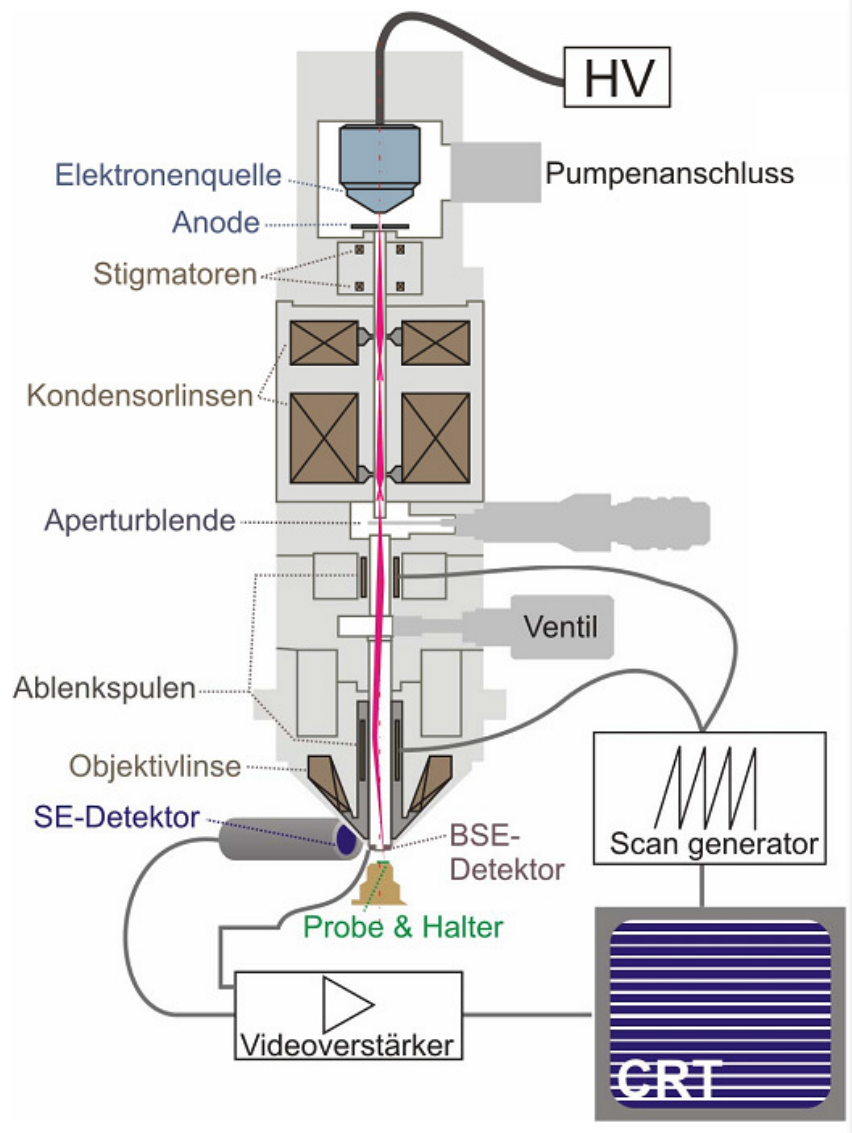
\includegraphics[scale=0.25]{AufbauREM.png}
    \captionof{figure}{Aufbau Raster-Elektronenmikroskop}
    \label{image:aufbau}
\end{center}

\section{Wechselwirkung der Elektronen mit Materie}
\label{sec:elektrons}
Durch Wechselwirkung des Primärelektronenstrahls (PE) mit der Materie entstehen unterschiedliche Signale, welche in Abbildung \ref{image:signal} dargestellt sind.
\begin{center}
    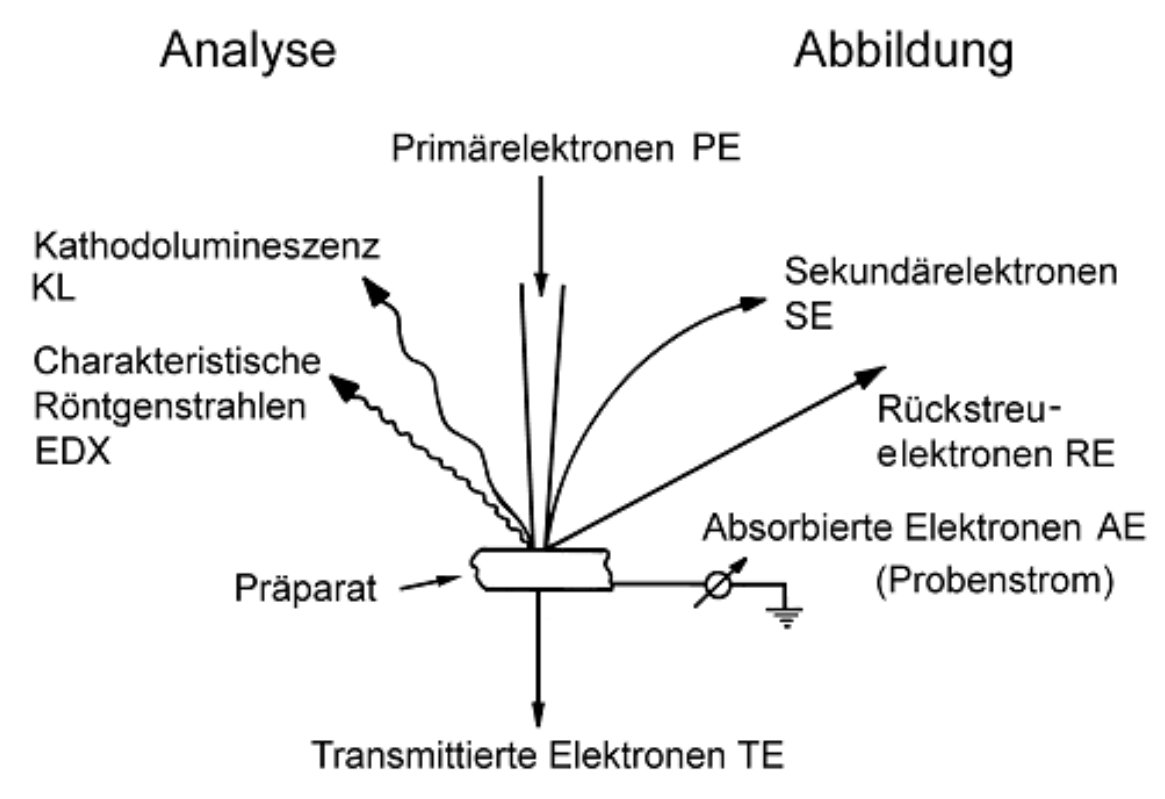
\includegraphics[scale=0.2]{Signalentstehung.png}
    \captionof{figure}{Signale eines REMs}
    \label{image:signal}
\end{center}
Das Volumen, in dem die Elektronen des Primärelektronenstrahls wechselwirken, heißt Streubirne oder Elektronendiffusionswolke, wobei die Reichweite vom gewählten Probenmaterial und der Anregungsspannung abhängt. 
\begin{center}
    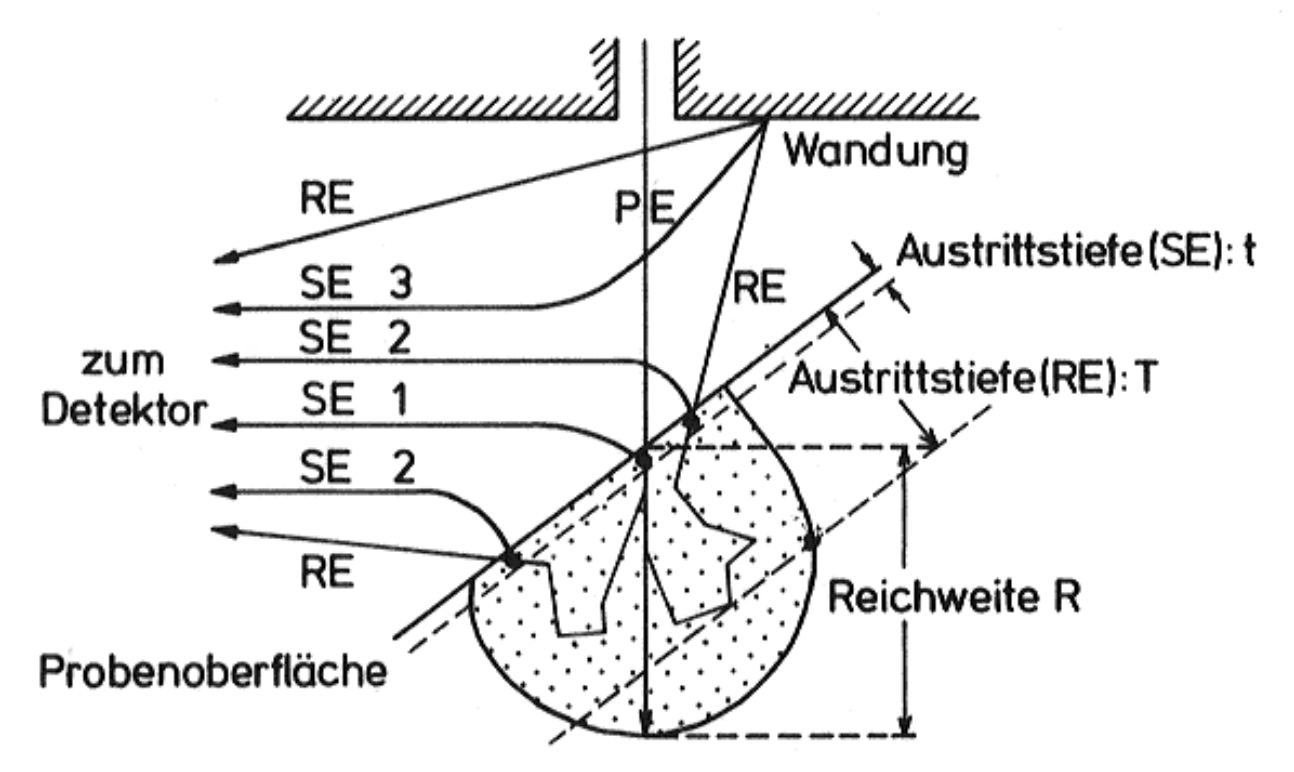
\includegraphics[scale=0.2]{Elektronendiffusionswolke.png}
    \captionof{figure}{Elektronendiffusionswolke}
    \label{image:wolke}
\end{center}
Durch Eindringen des PE entstehen durch unelastische Streuung langsame \textbf{\textit{Sekundärelektronen (SE)}} mit Energie < \SI{50}{\electronvolt} mit wahrscheinlichster Energie $\left\langle E\right\rangle=\SI{2,5}{\electronvolt}$, welche aus der $t =$ 1-\SI{10}{\nano\metre} stammen und zur Hochauflösung des REM führen. \citep{RasterEM} Somit tragen SE maßgeblich zu den dem sogenannten \textit{Topografiekontrast} bei. \citep{WikipolyREM}\\

Elektronen, welche elastisch an Atomkerne gestreut werden und diesen unter großen Winkel verlassen, werden als \textbf{\textit{Rückstoßelektronen (RE)}}. REs haben dabei eine Energie > \SI{50}{\electronvolt}, worunter auch schnellere SE fallen, aber diese sind von REs nicht unterscheidbar sind. Dabei stammen die ausgelösten REs aus einer Materialtiefe $T=$0,1-\SI{1}{\micro\metre} und sind somit verantwortlich für den \textit{Materialkontrast}. Auch hängt die Ausbeute der REs von der Kernladungszahl des Materials ab. \citep{RasterEM} \citep{WikipolyREM} Die REs können auch beim Austreten weitere SEs erzeugen, was man gut Anhand des \textit{Kantenkontrast} erkennen kann. \citep{RasterEM} \\

SE werden dann in Gruppen unterteilt:
\begin{itemize}
    \item \textbf{SE1:} Aus PE im Material erzeugte SEs
    \item \textbf{SE2:} Aus RE im Material erzeugte SEs 
    \item \textbf{SE3:} Aus RE außerhalb des Materials erzeugte SEs\\   
\end{itemize}

Bis zu einer Reichweite von $R=\SI{500}{\nano\metre}$ entsteht eine Wechselwirkung des PE-Strahls mit der Probe, wobei Elektronen aus der Atomhülle geschlagen werden. Dabei fallen Elektronen aus höheren Zuständen nach und es entsteht dabei Röntgenstrahlung, wobei diese Strahlung charakteristisch für das jeweilige Element ist. Die emittierende Strahlung kann dann noch ein Elektron aus einer höheren Schale herausschlagen, was als Auger-Elektron registriert wird. Bei Kernen mit kleiner Ordnungszahl ($Z$<20) dominiert die Emission von Auger-Elektronen, bei
höheren Ordnungszahlen überwiegt die Emission von charakteristischer Röntgenstrahlung.

\section{Detektoren}
\label{sec:detect}

\subsection*{Everheart-Thornley-Detektor}
\label{sub:etDetect}
\begin{center}
    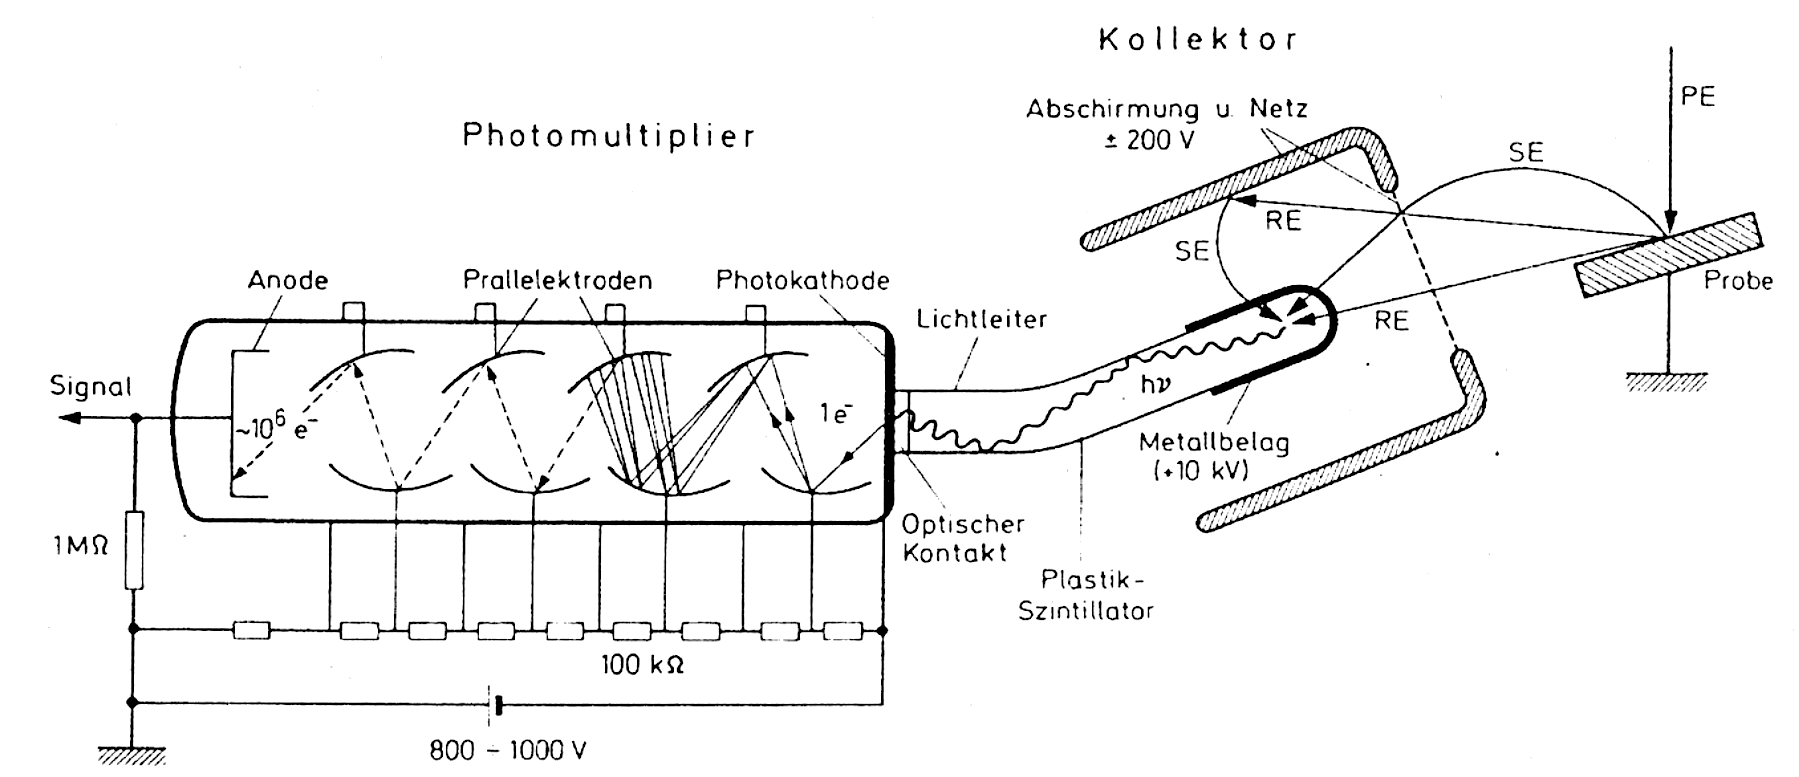
\includegraphics[scale=0.23]{Everheart-Thornley.png}
    \captionof{figure}{Everheart-Thornley-Detektor}
    \label{image:etDetect}
\end{center}
Der Everheart-Thornley-Detektor ist eine Kombination aus Szintillator und Photomultiplier (siehe Abb. \ref{image:etDetect}), welcher zur Detektierung von SEs und REs dient. Die ausgelösten Ses werden dabei von einem Netz des Kollektors mit positiver Spannung angesaugt (mit negativer Spannung können SEs zurückgehalten werden $\Rightarrow$ nur REs im Signal). Schnelle REs, welche einen wesentlich höhere Energie wie SEs haben, passieren das Netz in beiden Fällen. Zwischen Netz und einer \SI{50}{\nano\metre} dünnen leitende Metallschicht auf der Oberfläche des Plastik-Szintillators liegt eine Spannung von \SI{10} {\kilo\volt}, welche die Elektronen zum Szintillator beschleunigen. Dabei entstehen im Szintillator eine große Elektron-Loch-Paar, welcher proportional zur Spannung zwischen Probe und Kollektor und der Neigung der Probe zum Kollektor ist. Die Rekombination dieser Paare erzeugt Lichtquanten, wobei ein großer Teil strahlungslos rekombiniert. Dabei werden die erzeugten Lichtquanten durch Totalreflexion in Richtung des Photomultiplier abgelenkt. Auf der Photokathode wird dann durch das Quant ein Elektron ausgelöst, wobei diese durch eine Prallelektrode auf \SI{100}{\electronvolt} beschleunigt und Spannungsimpulse induzieren, welche wiederum elektronisch verstärkt werden können. Dabei führt jedes einfallende SE mindestens zu einem Spannungsimpuls. Die Spannungsimpuls sorgen dann für einen Steuerung der Bildschirmhelligkeit. \citep{RasterEM}

\subsection*{Halbleiterdetektor}
\label{sub:halbDetect}
\begin{center}
    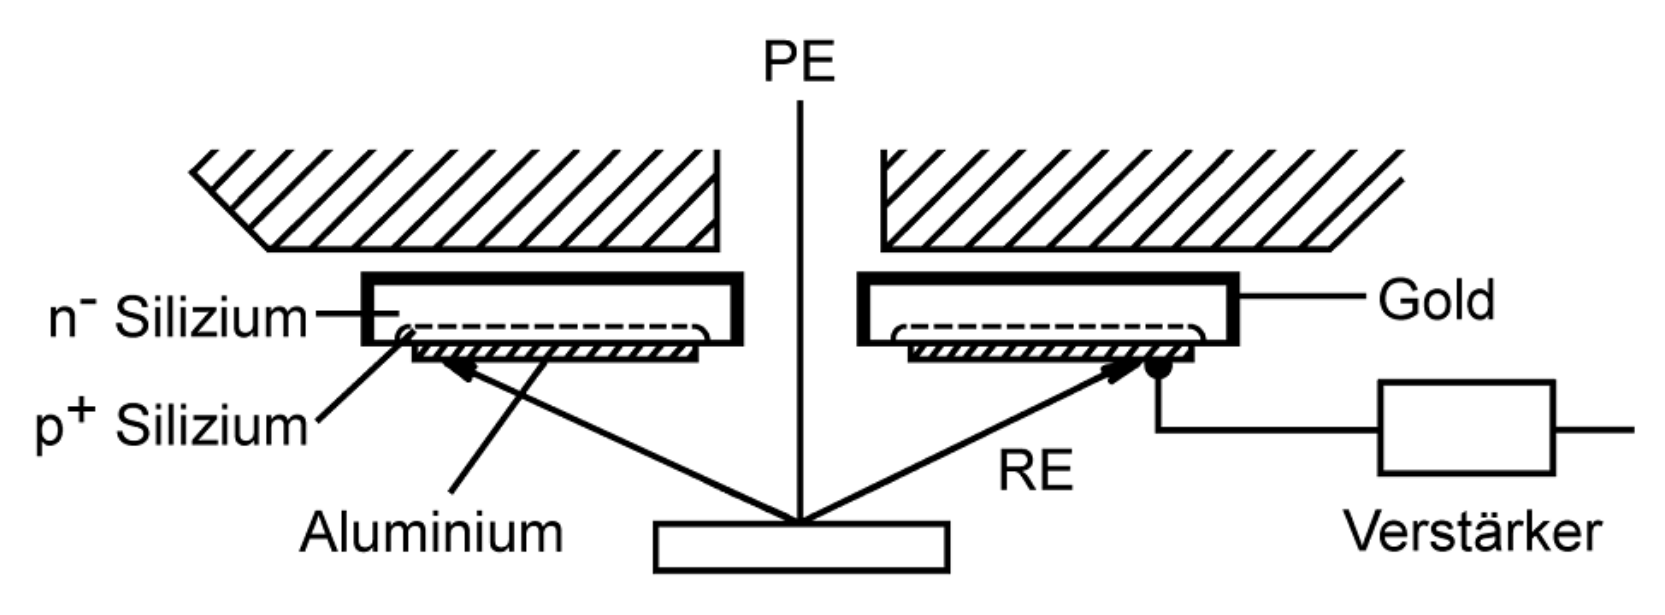
\includegraphics[scale=0.2]{Halbleiterdetektor.png}
    \captionof{figure}{Halbleiterdetektor}
    \label{image:halbDetect}
\end{center}
Halbleiterdetektor sind im Grunde Dioden, welche in Sperrrichtung betrieben werden. Dafür eigenen sich diese Detektoren besonders gut für die Untersuchung von REs. Durch das Aluminium wird verhindert, dass Lichtquanten mitdetektiert werden. Auch werden langsame SEs von der Al-Schicht absorbiert. Die REs erzeugen im Leiter Elektron-Loch-Paare, welche dann über den p-n-Übergang diffundieren können, wobei es dort zu Rekombinationen in der jeweiligen Schicht kommt oder getrennt werden. Durch die Trennung der Elektron-Loch-Paare fließt durch den Leiter ein Strom, welcher weiter verstärkt wird und wiederum zur Helligkeitsmodulation dient. Durch seine flache Bauform kann der Halbleiterdetektor nahe an der Probe angebracht werden und füllt zum Gegensatz von (\ref{sub:etDetect}) einen großen Raumwinkel aus. \citep{RasterEM}
\begin{center}
    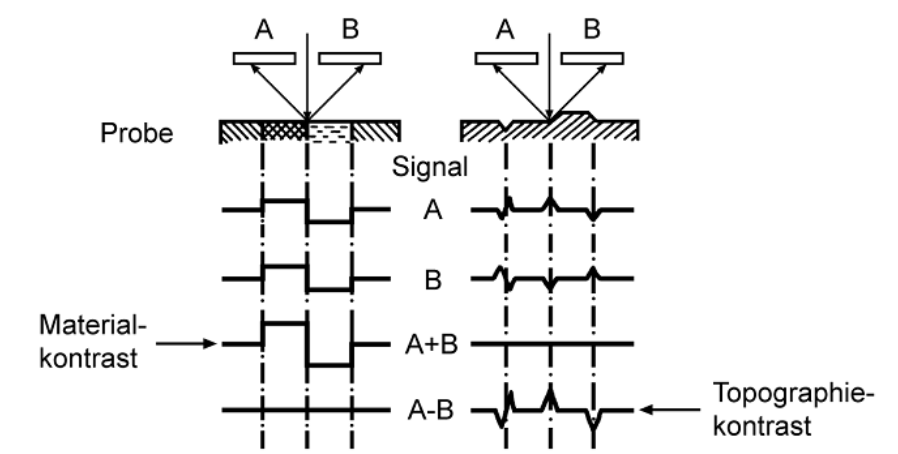
\includegraphics[scale=0.3]{Modi.png}
    \captionof{figure}{Combo- und Topomode}
    \label{image:modi}
\end{center}
Der Halbleiterdetektor kann dabei in verschiedenen Modi betrieben werden (siehe Abb. \ref{image:modi}). Den Combo- (Materialkontrast) und den Topo-Mode (Topografiekontrast).
Weiterhin kann das verwendete Elektronenmikroskop in Praktikum den sogenannten Shadow-Mode, welcher es ermöglicht Combo- und Topo-Mode gleichzeitig zu betrachten. Möglich gemacht wird dies mit Hilfe es dritten Detektor, welcher leicht schräg angewinkelt ist (siehe Abb. \ref{image:halbDetect}).

\subsection*{Si(Li)-Detektor und SDD-Detektor}
\label{sub:siliDetect}
Bei einem Si-Detektor handelt es sich im Grunde um eine in Sperrrichtung betriebenen Silizium-Diode. Dabei Wird bei einer angelegten Sperrspannung eine ladungsträgerfreie Zone(intrinsische Zone) erzeugt. Durch die einfallenden Röntgenquanten werden Elektron-Loch-Paare erzeugt, die durch die angelegte Sperrspannung zu den Elektroden getrennt werden und dabei einen Spannungsimpuls verursachen. Für höhere Effizienz wird die Si-Diode mit Lithium dotiert, womit der Si(Li)-Detektor entsteht. Das Lithium fungiert als Donator und erzeugt mit den p-leitenden Charakter des Siliziums einen p-i-n-Übergang. Um das Driften der Lithium-Ionen zu verhindern, muss der Si(Li)-Detektor permanent gekühlt werden. \citep{RasterEM}
\begin{center}
    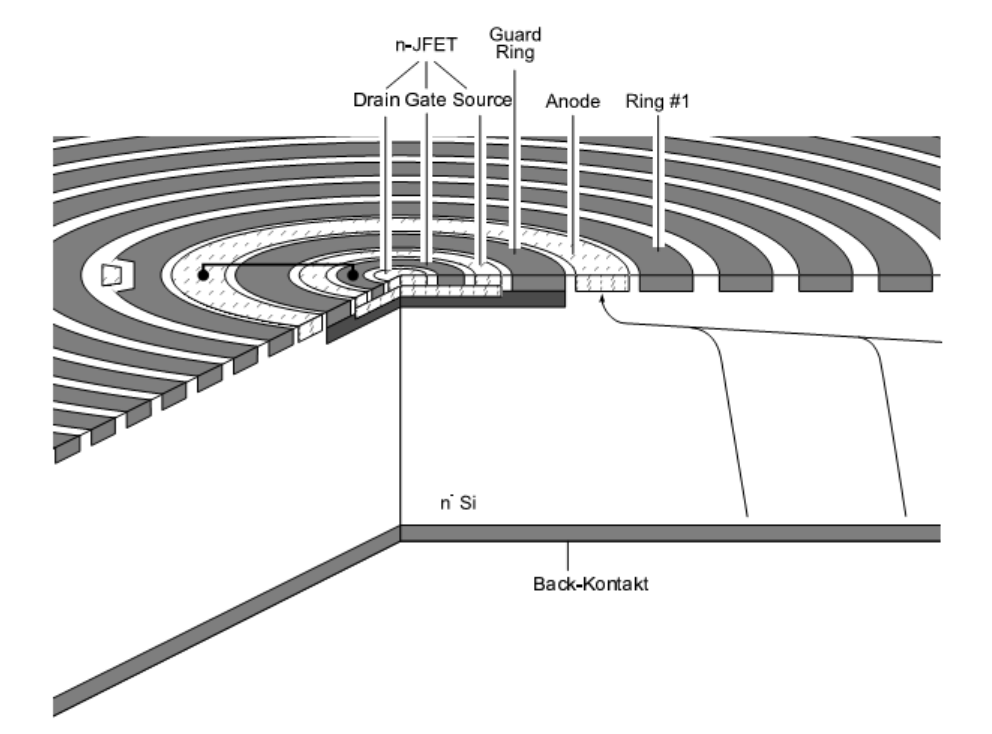
\includegraphics[scale=0.2]{Wafer.png}
    \captionof{figure}{SDD-Detektor}
    \label{image:sddDetect}
\end{center}
Ein Silizium Drift Detektor (SDD) besteht nur aus einem Silizium-Wafer, der mit ringförmigen Elektroden auf der obereren Seite besitzt. Hierbei weist die angelegte Spannung einen Gradienten auf, welcher von Innen nach Außen zunimmt. Als Signalverstärker fungiert ein Feldeffekt Transistor (FET) im Zentrum des Wafers. Der SDD besitzt dabei keine klassische Diodenstruktur und besteht dabei aus zwei gegenüberliegenden p+ dotierten Schichten mit n- dotierter Rückseite als Sammelelektrode. Bei Sperrspannung entsteht auch wieder eine ladungsträgerfreie Zone und ein Potenzialminimum im Zentrum des Wafers, wobei somit ein Spannungsgradient erzeugt wird, der die Elektronen (aus Elektron-Loch-Paar erzeugt durch Röntgenquant) zur Anode leitet und die Löcher zu den Driftringe (siehe Abb. \ref{image:drift}).
\begin{center}
    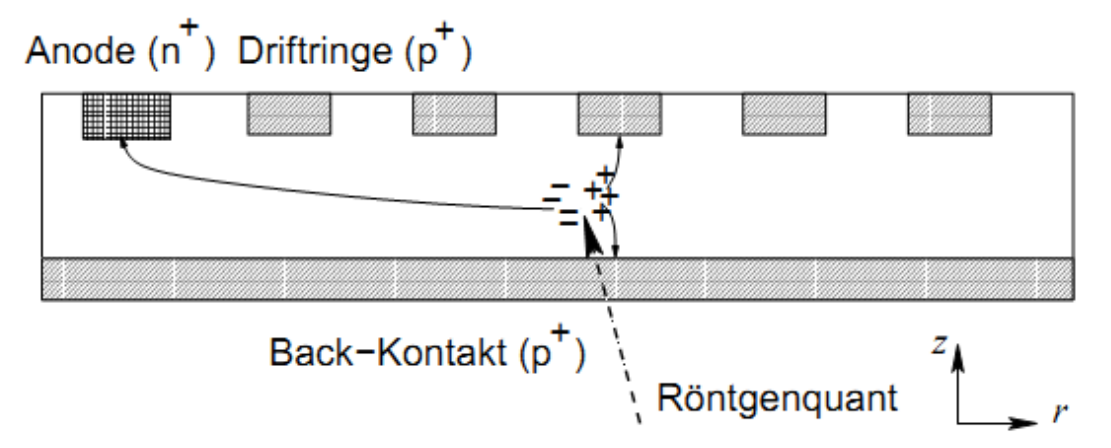
\includegraphics[scale=0.2]{WaferFunk.png}
    \captionof{figure}{Driftfeld SDD-Detektor}
    \label{image:drift}
\end{center}
Der SDD nimmt dabei das klassische Röntgenspektrum (Bremsspektrum, etc.) auf, wobei dabei die $K_\alpha$ für die praktische Analyse am wichtigsten ist, da diese am wahrscheinlichsten entsteht. Die Aufnahme der Spektrallininen kann dabei über wellenlängendispersiv oder energiedispersiv aufgenommen werden. Dabei wird bei einem wellenlängendispersiven Spektrometer (WDS) jeweils auf eine Spektrallinie (mit Hilfe eines Analysatorkristall) direkt eingestellt, wodurch eine genaue Bestimmung der Intensität möglich ist. Bei einem energiedispersiven Spektrometer (EDS) wird simultan das gesamte Röntgenspektrum erfasst wird, was eine gute Übersicht über die auftretenden Linien gibt. Wichtig zu erwähnen ist, dass ein EDS auch bei rauhen Oberflächen ohne Intensitätsabnahme verwendet werden kann, wobei die Messung nur qualitativ ist. Auch ist zu beachten, dass bei einem EDS Überlappungen auftreten können. \citep{RasterEM}

\section{Abbildungsfehler und Kontraste}
\label{sec:imageErrorKontrast}

    % 3.Kapitel Protokoll
    % Charlotte Geiger - Manuel Lippert - Leonard Schatt
% Physikalisches Praktikum

% 3.Kapitel  Protokoll

% Variables
\def\skalierung{0.65}

\chapter{Messprotokoll}
\label{chap:protokoll}

Das Messprotokoll wurde am Versuchstag handschriftlich erstellt und hier als
PDF-Datei eingefügt. Dabei wurden Durchführung und Aufbau schon vorher in dieses
Dokument beschrieben, je nachdem. test

%\centering

% Einbindung des Protokolls als pdf (mit Seitenzahl etc.)
% Erste Seite mit Überschrift
%\includepdf[pages = 1, landscape = false, nup = 1x1, scale = \skalierung , pagecommand={\thispagestyle{empty}\chapter{Protokoll}}]
%            {03 Protokoll/Protokoll.pdf}
% Restliche Seiten richtig skaliert
\includepdf[pages = 2-, landscape = false, nup = 1x1, scale = \skalierung , pagecommand={}]
            {03-Protokoll/ProtokollSP.pdf}

    % 4.Kapitel Versuchsauswertung
    % 4. Versuchsauswertung

\chapter{Auswertung und Diskussion}
\label{chap:versuchsauswertung}

% Text

% Input der Teilauswertung je nach Produktion der Nebendateien ohne Ordner
% Teilauswertung X

\section{Teilauswertung X}
% Teilauswertung 4
\section{Lebenszeitmessung}
\label{sec:lebenszeit}

CFP1-c1 5.008 2.9295095907141993 \\
CFP2-c1 5.008 2.86328777266995 \\
CFP3-c1 5.008 2.864972335683961 \\
YFP1-c2 5.008 3.25925836091248 \\
YFP2-c2 5.008 3.4119299746334164 \\
YFP3-c2 5.008 3.3295197646160584 \\

% etc.

    % 5.Kapitel Fazit
    % Charlotte Geiger - Manuel Lippert - Leonard Schatt
% Physikalisches Praktikum

% 5. Kapitel Einleitung

\chapter{Fazit}
\label{chap:fazit}

% Platz für Text

    % Anhang
    \chapter{Peaks für den Depolarisationsgrad}
\begin{figure}[h]
  \centering
  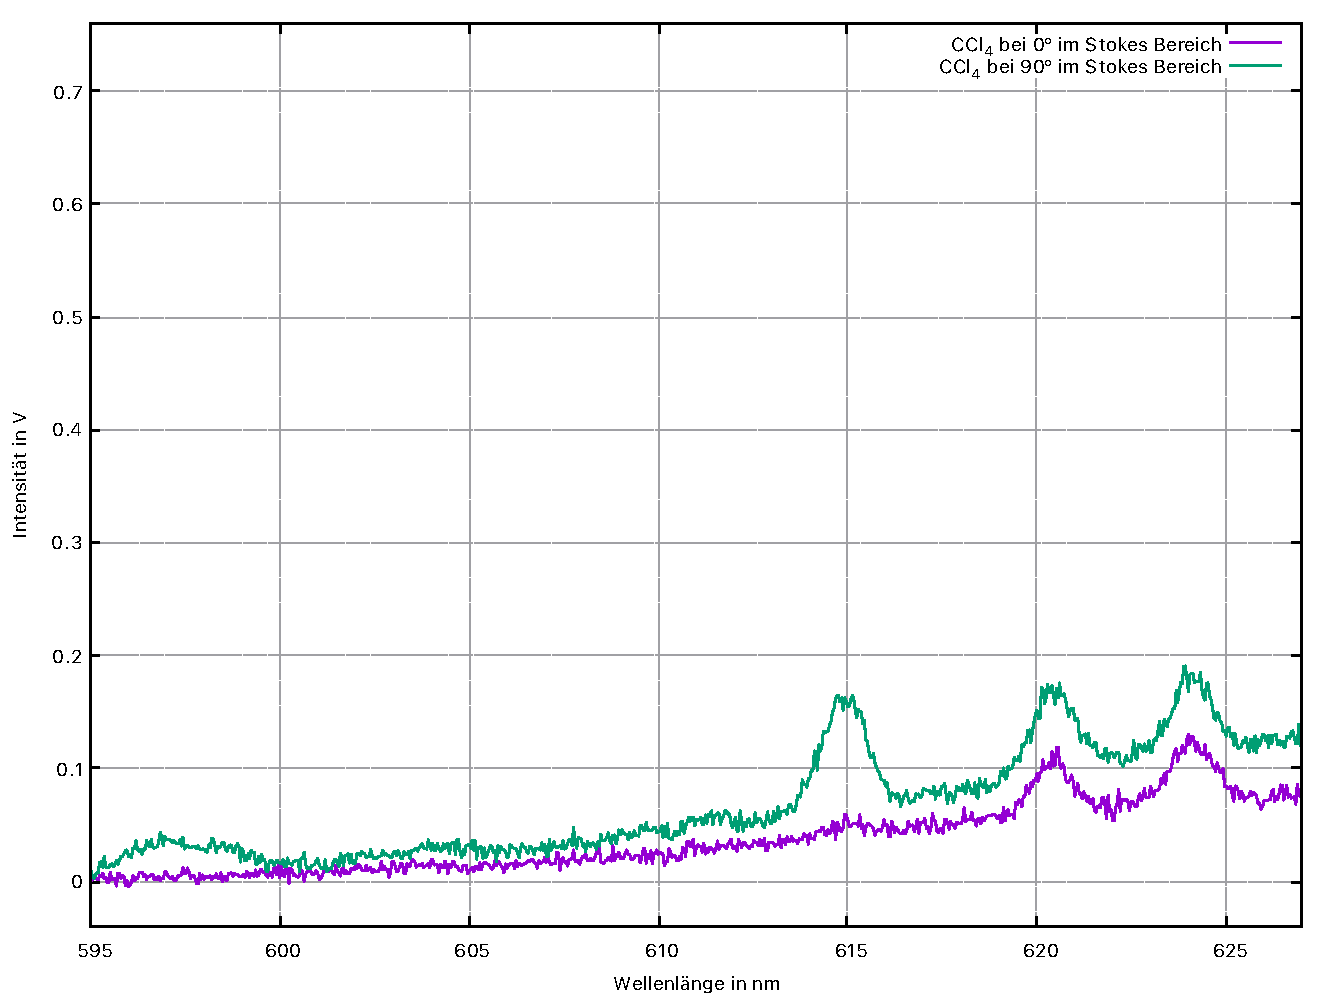
\includegraphics[scale=0.45]{Bilder/Verbesserung_Auswertung/ccl4_stokes.pdf}
  \caption{Spektrum von $CCl_4$, im Stokes Bereich bei 0° und 90° Polarisation.}
\end{figure}
\begin{figure}[h]
  \centering
  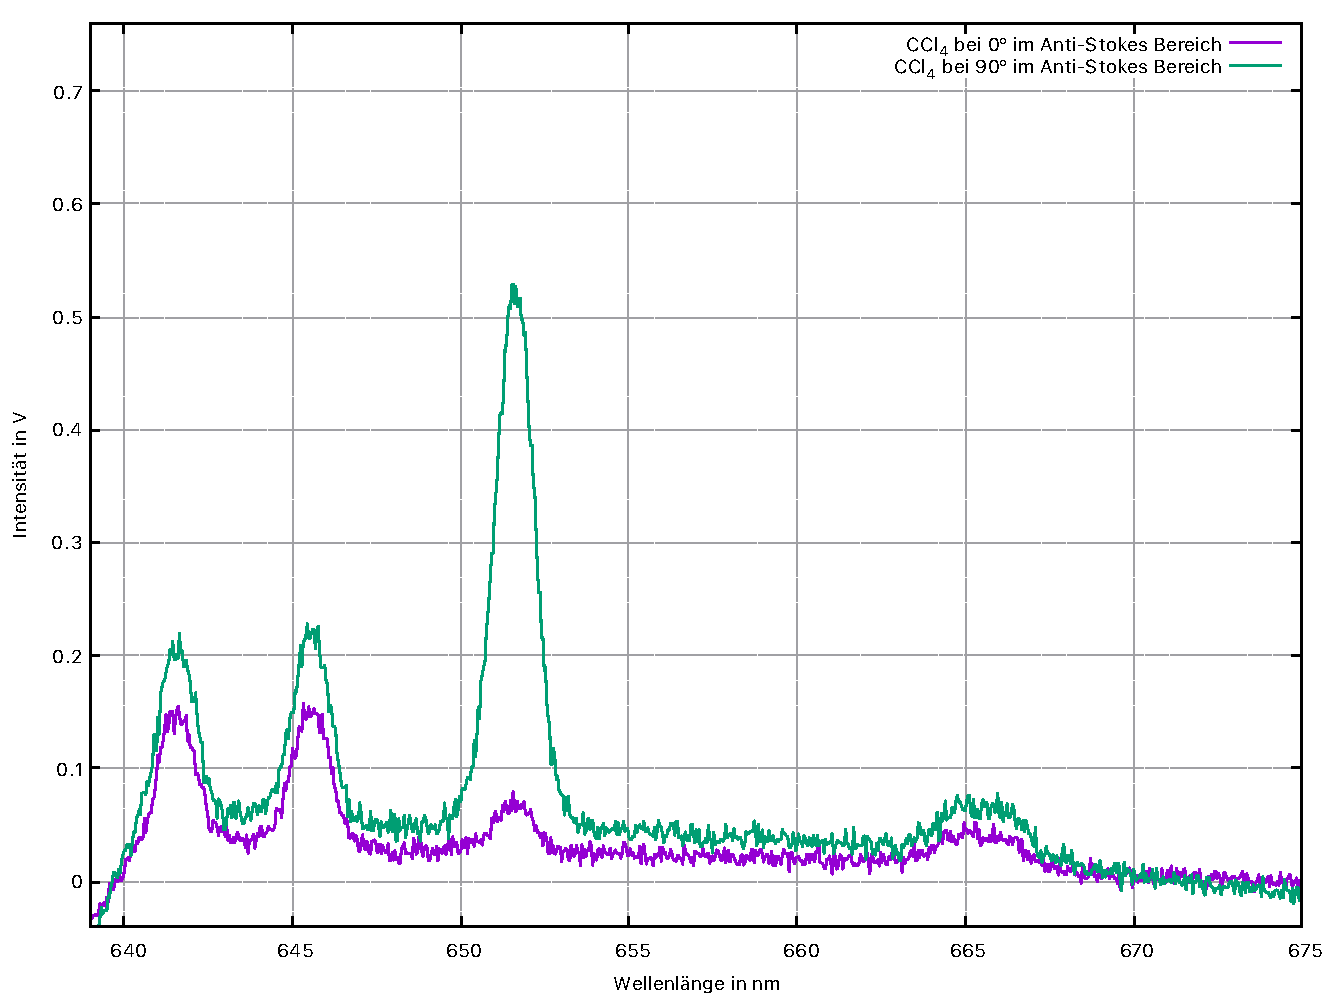
\includegraphics[scale=0.45]{Bilder/Verbesserung_Auswertung/ccl4_anti.pdf}
  \caption{Spektrum von $CCl_4$, im Anti-Stokes Bereich bei 0° und 90° Polarisation.}
\end{figure}
\begin{figure}[h]
  \centering
  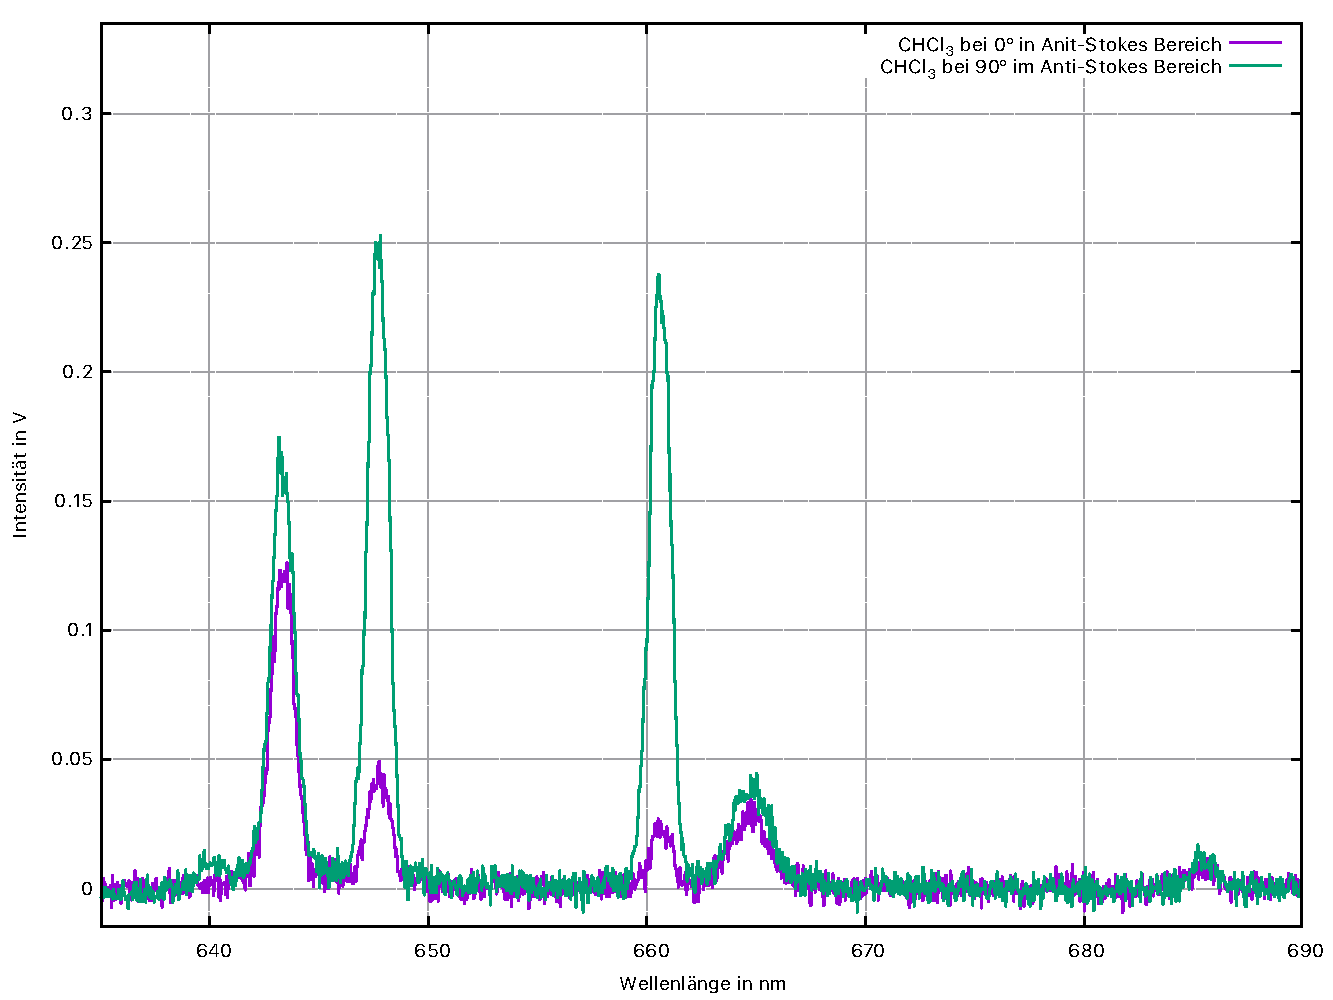
\includegraphics[scale=0.5]{Bilder/Verbesserung_Auswertung/chcl3_anti.pdf}
  \caption{Spektrum von $CHCl_3$, im Anti-Stokes Bereich bei 0° und 90° Polarisation.}
\end{figure}
\begin{figure}[h]
  \centering
  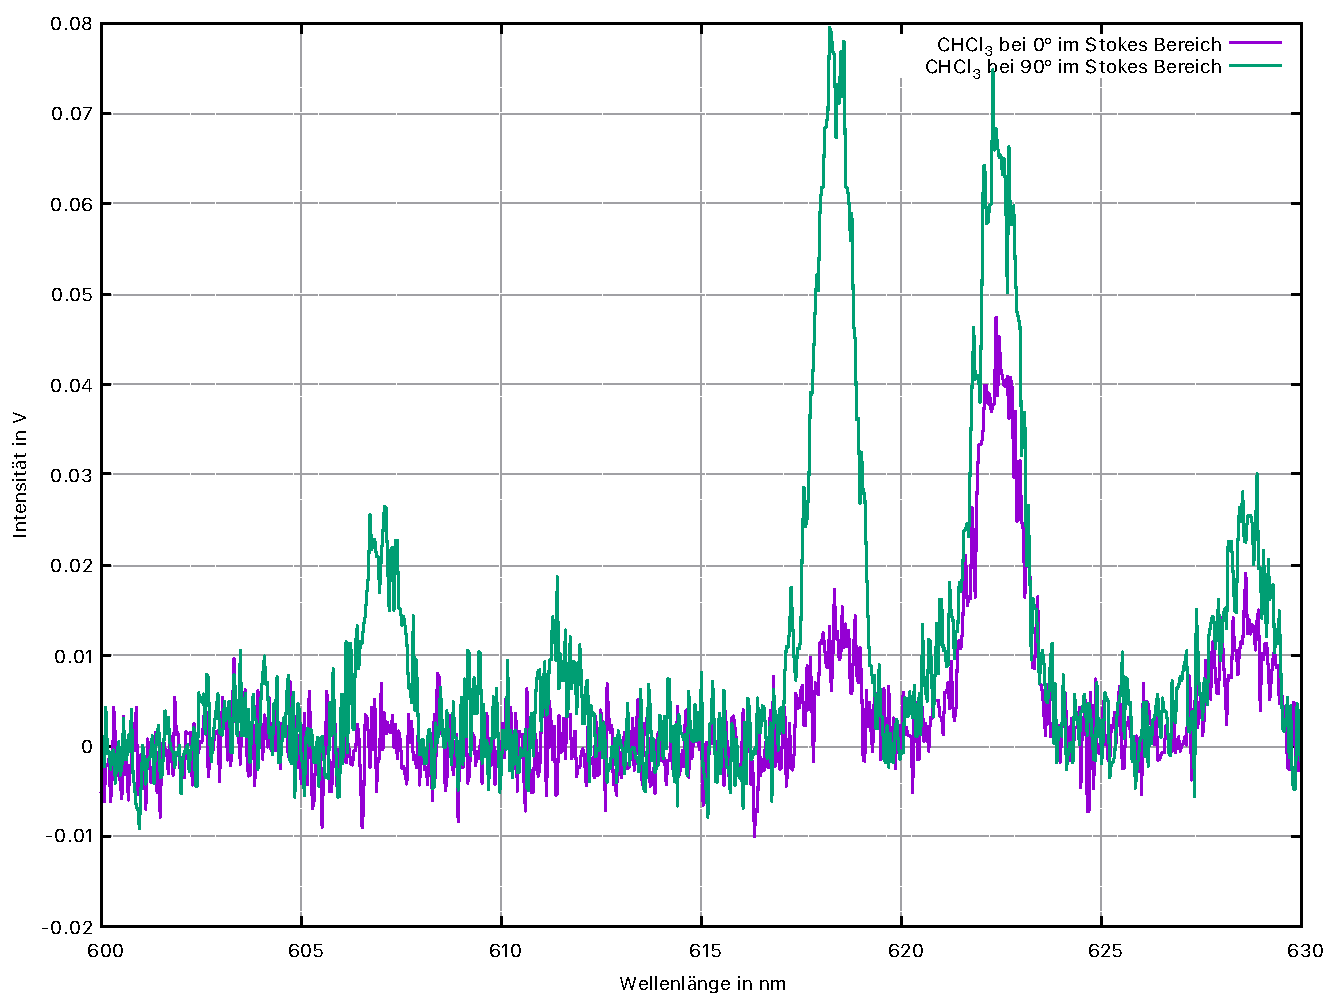
\includegraphics[scale=0.5]{Bilder/Verbesserung_Auswertung/chcl3_stokes.pdf}
  \caption{Spektrum von $CHCl_3$, im Stokes Bereich bei 0° und 90° Polarisation. In dem Bereich, indem es zur Überschneidung in der Wellenlänge bei den Peaks sowohl bei 0° als auch bei 90° kommt.}
\end{figure}

\chapter{Werte für Lage der Raman-Linien}
\begin{table}[h]
    \centering
    \begin{tabular}{c||c|c|c|c|c|c|c}
      \makecell{ $\lambda$ \\in nm} & $\nu$ in $\frac{1}{\text{cm}}$  & \makecell{ Fehler \\ $s_{\nu}$ in $\frac{1}{\text{cm}}$} & \makecell{Intensität\\ $0^{\circ}$ in V}  &  \makecell{Intensität\\ $90^{\circ}$ in V}  & \makecell{ Depolarisations- \\ grad $\rho$}  & \makecell{ Fehler \\ Depol. $s_{\rho}$} & Polarisation \\
      \hline
      643,3 & 270,4 & 12,1  & 0,1210 & 0,1688 & 0,7171 & 0,0365 & Depol. \\
      647,7 & 376,0 & 11,9  & 0,0470 & 0,2499 & 0,1879 & 0,0204 & Pol. \\
      660,7 & 679,8 & 11,5  & 0,0218 & 0,2279 & 0,0958 & 0,0220 & Pol. \\
      664,9 & 775,4 & 11,3  & 0,0281 & 0,0346 & 0,8123 & 0,1861 & Depol. \\
      685,3 & 1223,1 & 10,7  & 0,0088 & 0,0138 & 0,6359 & 0,4287 & Depol. \\  
    \end{tabular}
    \caption{Wellenlänge, Wellenzahl, Fehler der Wellenzahl, Intensität für 90° und 0°, Depolarisationsgrad und Fehler des Depolarisationsgrad für $CHCl_3$ im Anti-Stokes-Bereich.}
\end{table}
\begin{table}[h]
    \centering
    \begin{tabular}{c||c|c|c|c|c|c|c}
      \makecell{ $\lambda$ \\in nm} & $\nu$ in $\frac{1}{\text{cm}}$  & \makecell{ Fehler \\ $s_{\nu}$ in $\frac{1}{\text{cm}}$} & \makecell{Intensität\\ $0^{\circ}$ in V}  &  \makecell{Intensität\\ $90^{\circ}$ in V}  & \makecell{ Depolarisations- \\ grad $\rho$}  & \makecell{ Fehler \\ Depol. $s_{\rho}$} & Polarisation \\
    \hline
    643,3 & 270,4 & 12,1  & 0,1059 & 0,1747 & 0,6063 & 0,0335 & Depol. \\
    647,7 & 376,0 & 11,9  & 0,0434 & 0,2581 & 0,1681 & 0,0196 & Pol. \\
    659,9 & 661,5 & 11,5  & 0,0274 & 0,2651 & 0,1033 & 0,0190 & Pol. \\
    663,7 & 748,2 & 11,4  & 0,0320 & 0,0474 & 0,6754 & 0,1272 & Depol. \\
    671,4 & 921,0 & 11,1  & 0,0092 & 0,0181 & 0,5082 & 0,3092 & Depol. \\
  \end{tabular}%
\caption{Wellenlänge, Wellenzahl, Fehler der Wellenzahl, Intensität für 90° und 0°, Depolarisationsgrad und Fehler des Depolarisationsgrad für $CDCl_3$ im Anti-Stokes-Bereich.}
\end{table}\newpage
\begin{table}[h]
    \centering
    \begin{tabular}{c||c|c|c|c|c|c|c}
      \makecell{ $\lambda$ \\in nm} & $\nu$ in $\frac{1}{\text{cm}}$  & \makecell{ Fehler \\ $s_{\nu}$ in $\frac{1}{\text{cm}}$} & \makecell{Intensität\\ $0^{\circ}$ in V}  &  \makecell{Intensität\\ $90^{\circ}$ in V}  & \makecell{ Depolarisations- \\ grad $\rho$}  & \makecell{ Fehler \\ Depol. $s_{\rho}$} & Polarisation \\
      \hline
      639,0 & 165,8 & 12,3  & 0,0345 & 0,0655 & 0,5274 & 0,0863 & Depol. \\
      641,7 & 231,7 & 12,2  & 0,1201 & 0,7271 & 0,1652 & 0,0070 & Pol. \\
      655,1 & 550,4 & 11,7  & 0,0409 & 0,3626 & 0,1127 & 0,0139 & Pol. \\
      660,1 & 666,1 & 11,5  & 0,0841 & 0,1200 & 0,7007 & 0,0509 & Depol. \\  
    \end{tabular}%
    \caption{Wellenlänge, Wellenzahl, Fehler der Wellenzahl, Intensität für 90° und 0°, Depolarisationsgrad und Fehler des Depolarisationsgrad für $CHBr_3$ im Anti-Stokes-Bereich.}
\end{table}%
\begin{table}[h]
    \centering
    \begin{tabular}{c||c|c|c|c|c|c|c}
      \makecell{ $\lambda$ \\in nm} & $\nu$ in $\frac{1}{\text{cm}}$  & \makecell{ Fehler \\ $s_{\nu}$ in $\frac{1}{\text{cm}}$} & \makecell{Intensität\\ $0^{\circ}$ in V}  &  \makecell{Intensität\\ $90^{\circ}$ in V}  & \makecell{ Depolarisations- \\ grad $\rho$}  & \makecell{ Fehler \\ Depol. $s_{\rho}$} & Polarisation \\
      \hline
      641,5 & 226,8 & 12,2  & 0,1437 & 0,2009 & 0,7151 & 0,0306 & Depol. \\
      645,7 & 328,2 & 12,0  & 0,1472 & 0,2257 & 0,6520 & 0,0264 & Depol. \\
      651,7 & 470,8 & 11,8  & 0,0707 & 0,5163 & 0,1370 & 0,0098 & Pol. \\
      665,5 & 789,0 & 11,3  & 0,0381 & 0,0658 & 0,5793 & 0,0878 & Depol. \\  
    \end{tabular}
    \caption{Wellenlänge, Wellenzahl, Fehler der Wellenzahl, Intensität für 90° und 0°, Depolarisationsgrad und Fehler des Depolarisationsgrad für $CCl_4$ im Anti-Stokes-Bereich.}
  \end{table}%

    % Literatur
    \bibliographystyle{Libary/Auswertung.bst}
    \nocite{*}
    \bibliography{Libary/Auswertung.bib}

\end{document}